\begin{frame}
\frametitle{GPS}
\begin{itemize}
  \item Trilateration:  Knowing the distance from an unknown point to three known points yields the coordinates of the unknown point
  \item What if the distances are not known precisely?  
Answer:  Use 'pseudorange' instead, i.e., use signals traveling at speed of light and very accurate clocks
  \item What if the coordinates of the three points are not really known precisely?  Answer:  Use your best guess!
\end{itemize} 
\end{frame}

\begin{frame}
	\frametitle{Trilateration}
	\begin{figure}
	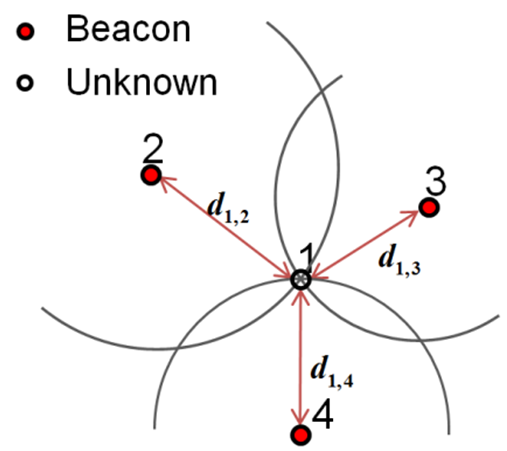
\includegraphics[width=0.5\textwidth]{graphics/trilateration.png}
\caption{Trilateration:  Distances to Three Beacons}
	\end{figure}
\end{frame}


\begin{frame}
	\frametitle{Pseudorange}
	\begin{itemize}
		\item distance = (speed of signal) $\times$ (time of signal flight)
		\begin{itemize}
			\item $\rho = c\Delta t$
		\end{itemize}
		\item Called 'pseudorange' because it is not a true range; it is only apparent due to inaccurate clocks
		\item By the same token, the coordinates of the transmitting satellites are also not known precisely, and so we could speak of 'pseudopositions' as well.   But nobody does that!
	\end{itemize}
\end{frame}

\begin{frame}
	\frametitle{Satellite Position}
	\begin{itemize}
		\item How do we know which satellite is transmitting? Answer:  Unique Pseudorandom Noise (PRN)
		\item How we know the position of the 
satellite at time of transmission?  Answer:
		\begin{itemize}
			\item Six Keplerian elements
			\item User receiver converts to WGS-84 X,Y,Z ECEF coordinates
		\end{itemize}
	\end{itemize}
\end{frame}

\begin{frame}
	\frametitle{Six Keplerian Elements}
	\begin{itemize}
		\item Eccentricity
		\item Semi-major axis
		\item Inclination
		\item Longitude of the ascending node
		\item Argument of periaspsis
		\item Mean anomaly
	\end{itemize}
\end{frame}

\begin{frame}
\frametitle{Keplerian Elements}
	\begin{figure}
	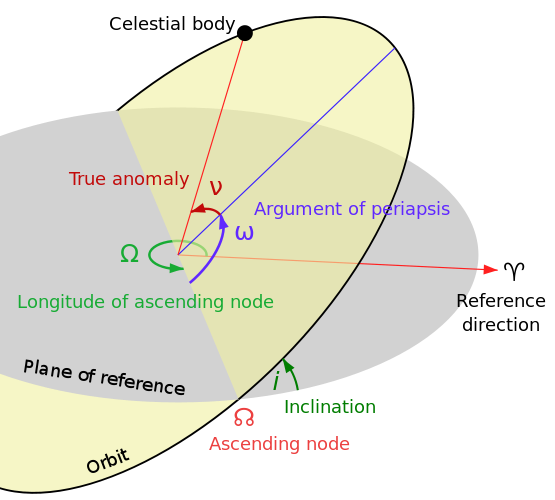
\includegraphics[width=0.75\textwidth,height=0.75\textheight]{graphics/555px-Orbit1_svg.png}
%	\caption{Keplerian Elements}
	\end{figure}
\end{frame}

\begin{frame}
\frametitle{Keplerian Elements}
	\begin{figure}
	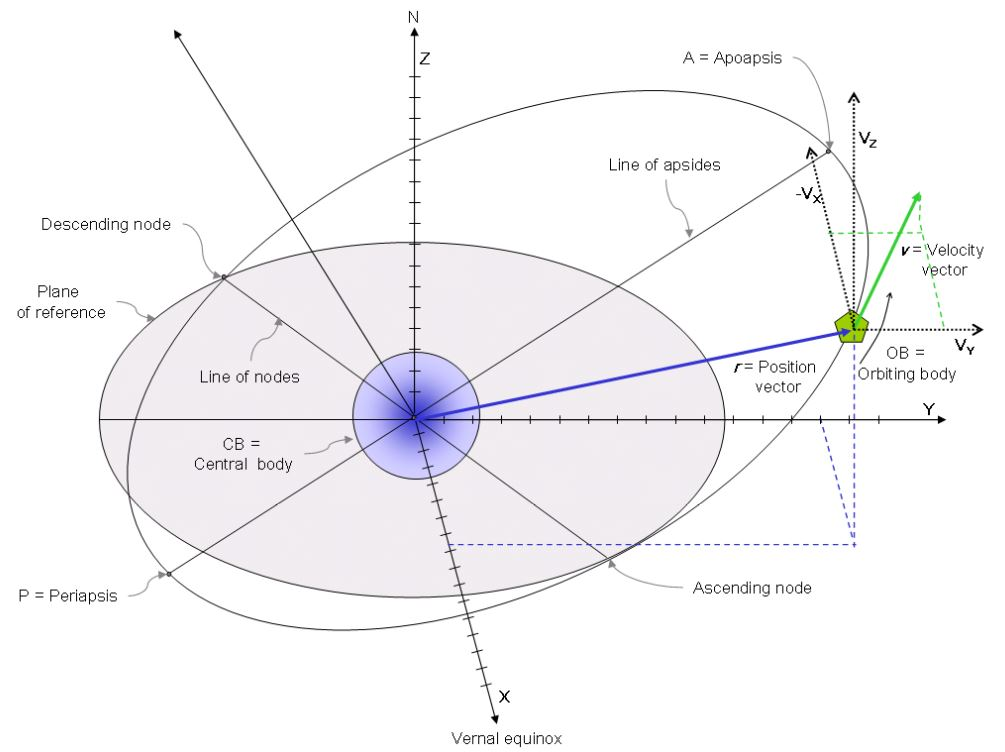
\includegraphics[width=0.80\textwidth,height=0.80\textheight]{graphics/keplerian_elements2.jpg}
%	\caption{Keplerian Elements}
	\end{figure}
\end{frame}

\begin{frame}
\frametitle{IS-GPS-200 Table 20-II}
\framesubtitle{1 of 2}
	\begin{figure}[h]
	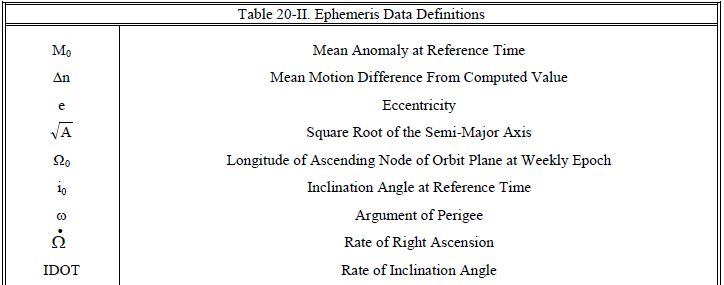
\includegraphics[width=0.8\textwidth]{graphics/table20-II-A.jpg}
%	\caption{Keplerian Elements}
	\end{figure}
\end{frame}

\begin{frame}
\frametitle{IS-GPS-200 Table 20-II}
\framesubtitle{2 of 2}
	\begin{figure}[h]
	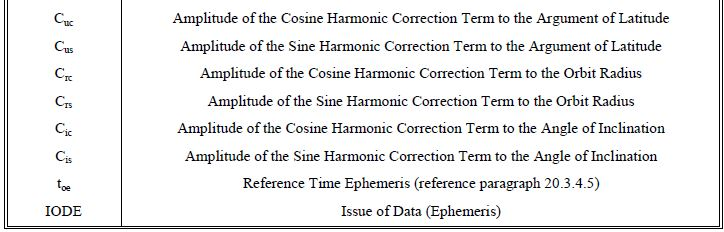
\includegraphics[width=0.8\textwidth]{graphics/table20-II-B.jpg}
%	\caption{Keplerian Elements}
	\end{figure}
\end{frame}

\begin{frame}
\frametitle{IS-GPS-200 Table 20-IV}
\framesubtitle{Elements of Coordinate Systems (1 of 3)}
	\begin{figure}[h]
	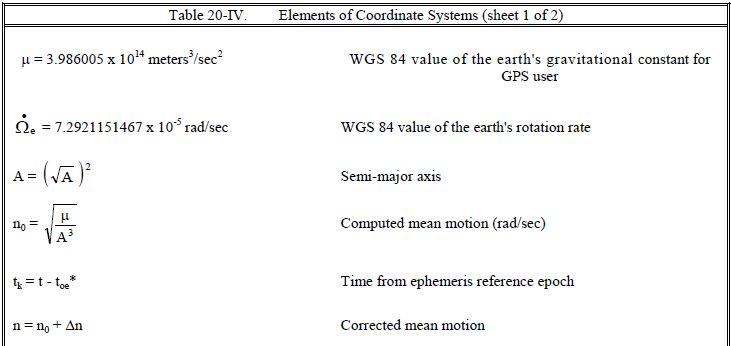
\includegraphics[width=0.8\textwidth]{graphics/table20-IV-A.jpg}
%	\caption{Keplerian Elements}
	\end{figure}
\end{frame}

\begin{frame}
\frametitle{IS-GPS-200 Table 20-IV}
\framesubtitle{Elements of Coordinate Systems (2 of 3)}
	\begin{figure}[h]
	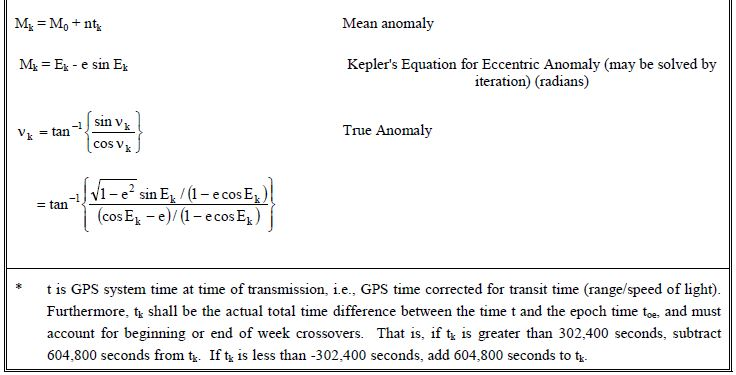
\includegraphics[width=0.8\textwidth]{graphics/table20-IV-B.jpg}
%	\caption{Keplerian Elements}
	\end{figure}
\end{frame}

\begin{frame}
\frametitle{IS-GPS-200 Table 20-IV}
\framesubtitle{Elements of Coordinate Systems (3 of 3)}
	\begin{figure}[h]
	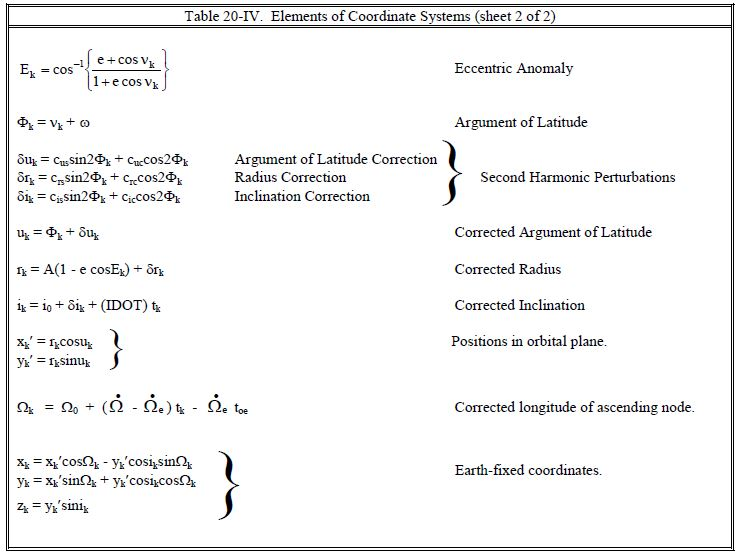
\includegraphics[width=0.8\textwidth]{graphics/table20-IV-C.jpg}
%	\caption{Keplerian Elements}
	\end{figure}
\end{frame}

